\section{ATMS NPP channel calculated brightness temperature comparisons}
%=======================================================================
\label{app:dtb}
This section lists the calculated brightness temperature differences for the various measaured SRFs with respect to the boxcar response. MonoRTM \cite{Clough_2005} was used to compute brightness temperatures for the ECMWF83 profile data set \cite{ECMWF_profile_set2,Matricardi_ECMWF564} at the frequencies shown in the NPP ATMS SRF plots of appendix \ref{app:srf}. These monochromatic brightness temperatures were then integrated over frequency to provide the channel brightness temperatures.

\newpage

% Note: the "[H]" placement option is allowed due to the use of the float package
%       in the preamble. I did this to avoid the
%        ! LaTeX Error: Too many unprocessed floats.
%       error due to the large number of figures.

\begin{figure}[H]
  \centering
  \includegraphics[scale=1]{graphics/dtb/atms_npp.ch1.TbStats.eps}
  \caption{NPP ATMS channel 1 calculated brightness temperature differences. \textbf{(Left)} $\Delta T_B$ as a function of the boxcar SRF $T_B$. \textbf{(Right)} Histogram of $\Delta T_B$ with respect to boxcar SRF $T_B$.}
  \label{fig:atms_npp.ch1.dtb}
\end{figure}

\begin{figure}[H]
  \centering
  \includegraphics[scale=1]{graphics/dtb/atms_npp.ch2.TbStats.eps}
  \caption{NPP ATMS channel 2 calculated brightness temperature differences. \textbf{(Left)} $\Delta T_B$ as a function of the boxcar SRF $T_B$. \textbf{(Right)} Histogram of $\Delta T_B$ with respect to boxcar SRF $T_B$.}
  \label{fig:atms_npp.ch2.dtb}
\end{figure}

\begin{figure}[H]
  \centering
  \includegraphics[scale=1]{graphics/dtb/atms_npp.ch3.TbStats.eps}
  \caption{NPP ATMS channel 3 calculated brightness temperature differences. \textbf{(Left)} $\Delta T_B$ as a function of the boxcar SRF $T_B$. \textbf{(Right)} Histogram of $\Delta T_B$ with respect to boxcar SRF $T_B$.}
  \label{fig:atms_npp.ch3.dtb}
\end{figure}

\begin{figure}[H]
  \centering
  \includegraphics[scale=1]{graphics/dtb/atms_npp.ch4.TbStats.eps}
  \caption{NPP ATMS channel 4 calculated brightness temperature differences. \textbf{(Left)} $\Delta T_B$ as a function of the boxcar SRF $T_B$. \textbf{(Right)} Histogram of $\Delta T_B$ with respect to boxcar SRF $T_B$.}
  \label{fig:atms_npp.ch4.dtb}
\end{figure}

\begin{figure}[H]
  \centering
  \includegraphics[scale=1]{graphics/dtb/atms_npp.ch5.TbStats.eps}
  \caption{NPP ATMS channel 5 calculated brightness temperature differences. \textbf{(Left)} $\Delta T_B$ as a function of the boxcar SRF $T_B$. \textbf{(Right)} Histogram of $\Delta T_B$ with respect to boxcar SRF $T_B$.}
  \label{fig:atms_npp.ch5.dtb}
\end{figure}

\begin{figure}[H]
  \centering
  \includegraphics[scale=1]{graphics/dtb/atms_npp.ch6.TbStats.eps}
  \caption{NPP ATMS channel 6 calculated brightness temperature differences. \textbf{(Left)} $\Delta T_B$ as a function of the boxcar SRF $T_B$. \textbf{(Right)} Histogram of $\Delta T_B$ with respect to boxcar SRF $T_B$.}
  \label{fig:atms_npp.ch6.dtb}
\end{figure}

\begin{figure}[H]
  \centering
  \includegraphics[scale=1]{graphics/dtb/atms_npp.ch7.TbStats.eps}
  \caption{NPP ATMS channel 7 calculated brightness temperature differences. \textbf{(Left)} $\Delta T_B$ as a function of the boxcar SRF $T_B$. \textbf{(Right)} Histogram of $\Delta T_B$ with respect to boxcar SRF $T_B$.}
  \label{fig:atms_npp.ch7.dtb}
\end{figure}

\begin{figure}[H]
  \centering
  \includegraphics[scale=1]{graphics/dtb/atms_npp.ch8.TbStats.eps}
  \caption{NPP ATMS channel 8 calculated brightness temperature differences. \textbf{(Left)} $\Delta T_B$ as a function of the boxcar SRF $T_B$. \textbf{(Right)} Histogram of $\Delta T_B$ with respect to boxcar SRF $T_B$.}
  \label{fig:atms_npp.ch8.dtb}
\end{figure}

\begin{figure}[H]
  \centering
  \includegraphics[scale=1]{graphics/dtb/atms_npp.ch9.TbStats.eps}
  \caption{NPP ATMS channel 9 calculated brightness temperature differences. \textbf{(Left)} $\Delta T_B$ as a function of the boxcar SRF $T_B$. \textbf{(Right)} Histogram of $\Delta T_B$ with respect to boxcar SRF $T_B$.}
  \label{fig:atms_npp.ch9.dtb}
\end{figure}

\begin{figure}[H]
  \centering
  \includegraphics[scale=1]{graphics/dtb/atms_npp.ch10.TbStats.eps}
  \caption{NPP ATMS channel 10 calculated brightness temperature differences. \textbf{(Left)} $\Delta T_B$ as a function of the boxcar SRF $T_B$. \textbf{(Right)} Histogram of $\Delta T_B$ with respect to boxcar SRF $T_B$.}
  \label{fig:atms_npp.ch10.dtb}
\end{figure}

\begin{figure}[H]
  \centering
  \includegraphics[scale=1]{graphics/dtb/atms_npp.ch11.TbStats.eps}
  \caption{NPP ATMS channel 11 calculated brightness temperature differences. \textbf{(Left)} $\Delta T_B$ as a function of the boxcar SRF $T_B$. \textbf{(Right)} Histogram of $\Delta T_B$ with respect to boxcar SRF $T_B$.}
  \label{fig:atms_npp.ch11.dtb}
\end{figure}

\begin{figure}[H]
  \centering
  \includegraphics[scale=1]{graphics/dtb/atms_npp.ch12.TbStats.eps}
  \caption{NPP ATMS channel 12 calculated brightness temperature differences. \textbf{(Left)} $\Delta T_B$ as a function of the boxcar SRF $T_B$. \textbf{(Right)} Histogram of $\Delta T_B$ with respect to boxcar SRF $T_B$.}
  \label{fig:atms_npp.ch12.dtb}
\end{figure}

\begin{figure}[H]
  \centering
  \includegraphics[scale=1]{graphics/dtb/atms_npp.ch13.TbStats.eps}
  \caption{NPP ATMS channel 13 calculated brightness temperature differences. \textbf{(Left)} $\Delta T_B$ as a function of the boxcar SRF $T_B$. \textbf{(Right)} Histogram of $\Delta T_B$ with respect to boxcar SRF $T_B$.}
  \label{fig:atms_npp.ch13.dtb}
\end{figure}

\begin{figure}[H]
  \centering
  \includegraphics[scale=1]{graphics/dtb/atms_npp.ch14.TbStats.eps}
  \caption{NPP ATMS channel 14 calculated brightness temperature differences. \textbf{(Left)} $\Delta T_B$ as a function of the boxcar SRF $T_B$. \textbf{(Right)} Histogram of $\Delta T_B$ with respect to boxcar SRF $T_B$.}
  \label{fig:atms_npp.ch14.dtb}
\end{figure}

\begin{figure}[H]
  \centering
  \includegraphics[scale=1]{graphics/dtb/atms_npp.ch15.TbStats.eps}
  \caption{NPP ATMS channel 15 calculated brightness temperature differences. \textbf{(Left)} $\Delta T_B$ as a function of the boxcar SRF $T_B$. \textbf{(Right)} Histogram of $\Delta T_B$ with respect to boxcar SRF $T_B$.}
  \label{fig:atms_npp.ch15.dtb}
\end{figure}

\begin{figure}[H]
  \centering
  \includegraphics[scale=1]{graphics/dtb/atms_npp.ch16.TbStats.eps}
  \caption{NPP ATMS channel 16 calculated brightness temperature differences. \textbf{(Left)} $\Delta T_B$ as a function of the boxcar SRF $T_B$. \textbf{(Right)} Histogram of $\Delta T_B$ with respect to boxcar SRF $T_B$.}
  \label{fig:atms_npp.ch16.dtb}
\end{figure}

\begin{figure}[H]
  \centering
  \includegraphics[scale=1]{graphics/dtb/atms_npp.ch17.TbStats.eps}
  \caption{NPP ATMS channel 17 calculated brightness temperature differences. \textbf{(Left)} $\Delta T_B$ as a function of the boxcar SRF $T_B$. \textbf{(Right)} Histogram of $\Delta T_B$ with respect to boxcar SRF $T_B$.}
  \label{fig:atms_npp.ch17.dtb}
\end{figure}

\begin{figure}[H]
  \centering
  \includegraphics[scale=1]{graphics/dtb/atms_npp.ch18.TbStats.eps}
  \caption{NPP ATMS channel 18 calculated brightness temperature differences. \textbf{(Left)} $\Delta T_B$ as a function of the boxcar SRF $T_B$. \textbf{(Right)} Histogram of $\Delta T_B$ with respect to boxcar SRF $T_B$.}
  \label{fig:atms_npp.ch18.dtb}
\end{figure}

\begin{figure}[H]
  \centering
  \includegraphics[scale=1]{graphics/dtb/atms_npp.ch19.TbStats.eps}
  \caption{NPP ATMS channel 19 calculated brightness temperature differences. \textbf{(Left)} $\Delta T_B$ as a function of the boxcar SRF $T_B$. \textbf{(Right)} Histogram of $\Delta T_B$ with respect to boxcar SRF $T_B$.}
  \label{fig:atms_npp.ch19.dtb}
\end{figure}

\begin{figure}[H]
  \centering
  \includegraphics[scale=1]{graphics/dtb/atms_npp.ch20.TbStats.eps}
  \caption{NPP ATMS channel 20 calculated brightness temperature differences. \textbf{(Left)} $\Delta T_B$ as a function of the boxcar SRF $T_B$. \textbf{(Right)} Histogram of $\Delta T_B$ with respect to boxcar SRF $T_B$.}
  \label{fig:atms_npp.ch20.dtb}
\end{figure}

\begin{figure}[H]
  \centering
  \includegraphics[scale=1]{graphics/dtb/atms_npp.ch21.TbStats.eps}
  \caption{NPP ATMS channel 21 calculated brightness temperature differences. \textbf{(Left)} $\Delta T_B$ as a function of the boxcar SRF $T_B$. \textbf{(Right)} Histogram of $\Delta T_B$ with respect to boxcar SRF $T_B$.}
  \label{fig:atms_npp.ch21.dtb}
\end{figure}

\begin{figure}[H]
  \centering
  \includegraphics[scale=1]{graphics/dtb/atms_npp.ch22.TbStats.eps}
  \caption{NPP ATMS channel 22 calculated brightness temperature differences. \textbf{(Left)} $\Delta T_B$ as a function of the boxcar SRF $T_B$. \textbf{(Right)} Histogram of $\Delta T_B$ with respect to boxcar SRF $T_B$.}
  \label{fig:atms_npp.ch22.dtb}
\end{figure}
